\documentclass[11pt]{article}
\usepackage[a3paper,portrait,margin=0.7in]{geometry}
\usepackage{tikz}
\usetikzlibrary{shapes.geometric, arrows.meta, positioning, calc, fit, backgrounds}
\usepackage{xcolor}
\usepackage{amsmath,amssymb}
\usepackage{microtype}
\usepackage{enumitem}
\usepackage{tcolorbox}
\tcbuselibrary{breakable, skins}
\usepackage{hyperref}
\hypersetup{colorlinks=true, linkcolor=teal, urlcolor=teal}

\setlist[itemize]{leftmargin=1.1em, topsep=1pt, itemsep=2pt, parsep=0pt}

% --- palette (light theme, matches project) ---
\definecolor{accentTeal}{HTML}{0E8B8B}
\definecolor{accentCyan}{HTML}{1FA1B5}
\definecolor{accentMagenta}{HTML}{B5197C}
\definecolor{accentGreen}{HTML}{0F9D58}
\definecolor{accentOrange}{HTML}{D6840B}
\definecolor{boxEdge}{HTML}{C9CDD3}
\definecolor{inkDim}{HTML}{5C6066}

\tcbset{
  sect/.style={
    enhanced, colback=white, colframe=accentTeal!55, boxrule=0.4pt,
    arc=4pt, left=10pt, right=10pt, top=8pt, bottom=8pt,
    fonttitle=\bfseries, coltitle=accentTeal, breakable,
    title filled=false,
    attach boxed title to top left={xshift=6mm, yshift=-2mm},
    boxed title style={
      colback=white, colframe=accentTeal!55, boxrule=0.4pt, arc=2pt
    }
  }
}

\tikzset{
  head/.style={draw=accentTeal, line width=0.8pt, rounded corners=3pt, fill=white,
               minimum width=2.4cm, minimum height=1.6cm, font=\small\bfseries},
  gear/.style={draw=#1, line width=0.9pt, fill=white, circle},
  arrow/.style={-{Stealth}, line width=1.1pt},
}

\pagestyle{empty}
\setlength{\parindent}{0pt}

\begin{document}

% ======================================================================
% TITLE BLOCK
% ======================================================================
\begin{center}
{\fontsize{28pt}{32pt}\selectfont\bfseries\color{accentTeal} BEYOND COMPONENTS}\\[2pt]
{\fontsize{14pt}{17pt}\selectfont\bfseries\color{black}
Recovering Scalable Algorithmic Circuits via Low-Rank Discovery}\\[4pt]
{\fontsize{11pt}{13pt}\selectfont\itshape\color{inkDim}`Core Engine'}
\end{center}
\vspace{6pt}

% ======================================================================
% SECTION 1 -- THE PROBLEM
% ======================================================================
\begin{tcolorbox}[sect, title=1. The problem --- the `atomic' fallacy]
\begin{minipage}[t]{0.32\linewidth}
\vspace{0pt}
\begin{center}
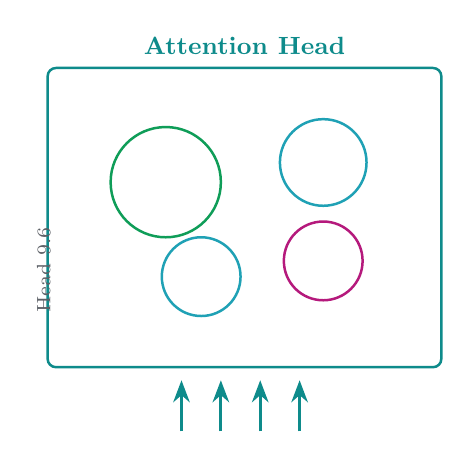
\begin{tikzpicture}
\node[draw=accentTeal, line width=0.9pt, rounded corners=3pt, fill=white,
      minimum width=5.0cm, minimum height=3.8cm] (head) {};
\node[above=1pt of head, font=\small\bfseries, color=accentTeal] {Attention Head};
\node[left=1pt of head, rotate=90, font=\scriptsize, color=inkDim] {Head 9.6};
\node[gear=accentGreen,   minimum size=1.4cm] at ($(head.center) + (-1.0, 0.45)$) {};
\node[gear=accentCyan,    minimum size=1.1cm] at ($(head.center) + (1.0, 0.7)$) {};
\node[gear=accentCyan,    minimum size=1.0cm] at ($(head.center) + (-0.55, -0.75)$) {};
\node[gear=accentMagenta, minimum size=1.0cm] at ($(head.center) + (1.0, -0.55)$) {};
\foreach \x in {-1.6, -0.6, 0.4, 1.4}{
  \draw[arrow, color=accentTeal] ($(head.south)!0.5!($(head.south) + (\x,0)$) + (0,-0.8)$)
        -- ($(head.south)!0.5!($(head.south) + (\x,0)$) + (0,-0.15)$);
}
\end{tikzpicture}
\end{center}
\end{minipage}%
\hfill
\begin{minipage}[t]{0.31\linewidth}
\vspace{6pt}
\textbf{\color{accentGreen}Polysemanticity} --- \emph{one component doing many jobs at once}.

Different-coloured gears = unrelated features all mixed inside the same head
(gender, number, punctuation, sentiment \dots).
\end{minipage}%
\hfill
\begin{minipage}[t]{0.33\linewidth}
\vspace{6pt}
Existing interpretability methods treat components (neurons, heads) as
\textbf{indivisible `atoms,'} which masks the true computational graph.

If one head handles gender, number, punctuation \emph{and} sentiment at once,
``this head is responsible for $X$'' is not a meaningful statement. We need
to go one level deeper.
\end{minipage}
\end{tcolorbox}

\vspace{4pt}

% ======================================================================
% SECTION 2 -- THE SOLUTION: SVD DECONSTRUCTION
% ======================================================================
\begin{tcolorbox}[sect, title=2. The solution --- SVD deconstruction]
\begin{minipage}[t]{0.48\linewidth}
\vspace{4pt}
\begin{center}
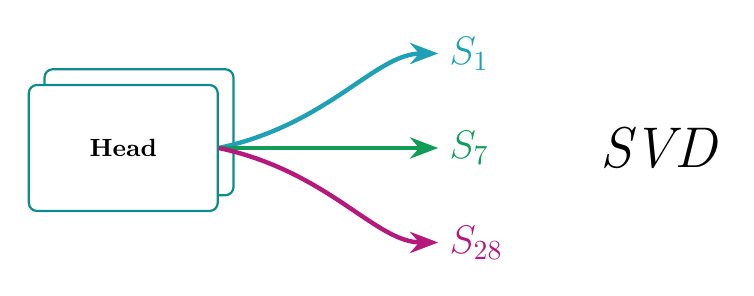
\begin{tikzpicture}
% stacked head boxes
\node[head, fill=white] (hd2) at (0.2, 0.2) {};
\node[head, fill=white] (hd) at (0, 0) {Head};

% arrows to S1, S7, S28
\draw[arrow, color=accentCyan, line width=1.6pt]
  (hd.east) .. controls +(1.4,0.3) and +(-0.8,0) .. (4.0, 1.2)
  node[right, font=\Large\itshape, color=accentCyan] {$S_{1}$};
\draw[arrow, color=accentGreen, line width=1.6pt]
  (hd.east) .. controls +(1.6,0.0) and +(-0.8,0) .. (4.0, 0.0)
  node[right, font=\Large\itshape, color=accentGreen] {$S_{7}$};
\draw[arrow, color=accentMagenta, line width=1.6pt]
  (hd.east) .. controls +(1.4,-0.3) and +(-0.8,0) .. (4.0, -1.2)
  node[right, font=\Large\itshape, color=accentMagenta] {$S_{28}$};

% SVD label
\node[font=\huge\itshape] at (6.8, 0) {SVD};

\end{tikzpicture}
\end{center}
\vspace{2pt}
\textbf{Mechanism.} SVD of the head's output-value matrix
$W_{OV}=U\Sigma V^{\top}$ gives an ordered basis. \textbf{Each row of $V^{\top}$
is one direction the head can write.} Top rows often correspond cleanly to a
single concept.
\end{minipage}%
\hfill
\begin{minipage}[t]{0.48\linewidth}
\vspace{4pt}
\begin{center}
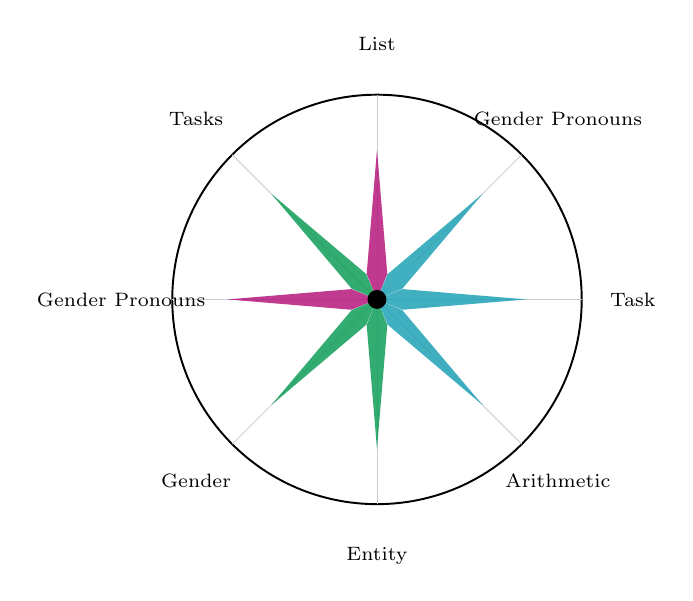
\begin{tikzpicture}
% compass rose
\draw[color=black, line width=0.7pt] (0,0) circle (2.6);
\foreach \a/\lbl in {90/List, 45/{Gender Pronouns}, 0/Task, -45/Arithmetic,
                     -90/Entity, -135/Gender, 180/{Gender Pronouns}, 135/Tasks}{
  \draw[color=boxEdge, line width=0.3pt] (0,0) -- ({2.6*cos(\a)}, {2.6*sin(\a)});
  \node at ({3.25*cos(\a)}, {3.25*sin(\a)}) {\scriptsize \lbl};
}
% 8-petal star
\foreach \a/\c in {90/accentMagenta, 0/accentCyan, -90/accentGreen, 180/accentMagenta,
                   45/accentCyan,  -45/accentCyan,  -135/accentGreen, 135/accentGreen}{
  \fill[\c, opacity=0.85]
    ({1.9*cos(\a)}, {1.9*sin(\a)}) --
    ({0.35*cos(\a-22)}, {0.35*sin(\a-22)}) --
    (0,0) --
    ({0.35*cos(\a+22)}, {0.35*sin(\a+22)}) -- cycle;
}
\fill[black] (0,0) circle (0.12);
\end{tikzpicture}
\end{center}
\vspace{2pt}
\begin{center}\small\itshape\color{inkDim}
Singular directions point to \emph{specific} concepts --- one direction, one named task.
\end{center}
\end{minipage}
\end{tcolorbox}

\vspace{4pt}

% ======================================================================
% SECTION 3 -- THE PROOF: SURGICAL CONTROL
% ======================================================================
\begin{tcolorbox}[sect, title=3. The proof --- surgical control]
\begin{minipage}[t]{0.31\linewidth}
\vspace{4pt}
\begin{center}
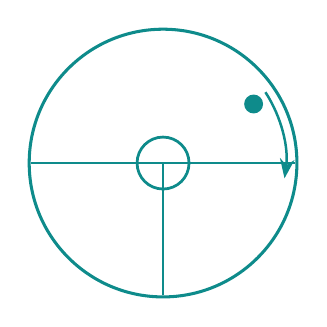
\begin{tikzpicture}
\draw[color=accentTeal, line width=1.1pt] (0,0) circle (1.7);
\draw[color=accentTeal, line width=1.0pt] (0,0) circle (0.33);
\draw[color=accentTeal, line width=1.0pt] (-1.68,0) -- (1.68,0);
\draw[color=accentTeal, line width=1.0pt] (0,-1.68) -- (0,0);
\draw[color=accentTeal, line width=0.9pt, -{Stealth}]
  (1.3,0.9) arc[start angle=33, end angle=-8, radius=1.6];
\fill[accentTeal] (1.15,0.75) circle (0.12);
\end{tikzpicture}\\[2pt]
\textbf{\small Steering wheel}\\
{\footnotesize\color{inkDim} Slider $=$ logit receptors --- one scalar $\alpha$ steers the model.}
\end{center}
\end{minipage}%
\hfill
\begin{minipage}[t]{0.31\linewidth}
\vspace{4pt}
\begin{center}
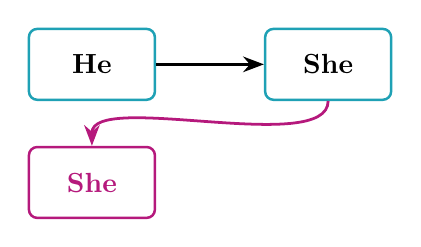
\begin{tikzpicture}
\node[draw=accentCyan, line width=0.9pt, rounded corners=3pt, fill=white,
      minimum width=1.6cm, minimum height=0.9cm] (he) at (0,0) {\bfseries He};
\node[draw=accentCyan, line width=0.9pt, rounded corners=3pt, fill=white,
      minimum width=1.6cm, minimum height=0.9cm] (she) at (3.0,0) {\bfseries She};
\draw[-{Stealth}, color=black, line width=1pt] (he) -- (she);
\node[draw=accentMagenta, line width=0.9pt, rounded corners=3pt, fill=white,
      minimum width=1.6cm, minimum height=0.9cm] (sh2) at (0,-1.5) {\bfseries\color{accentMagenta} She};
\draw[-{Stealth}, color=accentMagenta, line width=1pt]
  (she.south) .. controls +(0,-0.7) and +(0,0.7) .. (sh2.north);
\end{tikzpicture}\\[2pt]
\textbf{\small Before \& after}\\
{\footnotesize\color{inkDim} Pronoun flipped by adjusting \emph{just one scalar}.}
\end{center}
\end{minipage}%
\hfill
\begin{minipage}[t]{0.33\linewidth}
\vspace{4pt}
\begin{center}
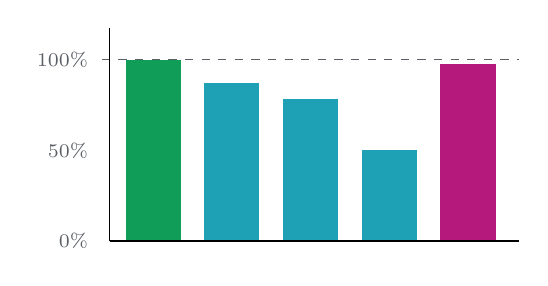
\begin{tikzpicture}
\draw[color=inkDim, dashed, line width=0.4pt] (-0.1,2.3) -- (5.2,2.3);
\node[left, font=\scriptsize, color=inkDim] at (-0.15,2.3) {100\%};
\node[left, font=\scriptsize, color=inkDim] at (-0.15,1.15) {50\%};
\node[left, font=\scriptsize, color=inkDim] at (-0.15,0)    {0\%};
\fill[accentGreen]   (0.2,0) rectangle (0.9,2.3);
\fill[accentCyan]    (1.2,0) rectangle (1.9,2.0);
\fill[accentCyan]    (2.2,0) rectangle (2.9,1.8);
\fill[accentCyan]    (3.2,0) rectangle (3.9,1.15);
\fill[accentMagenta] (4.2,0) rectangle (4.9,2.25);
\draw[color=black, line width=0.5pt] (0,0) -- (5.2,0);
\draw[color=black, line width=0.5pt] (0,0) -- (0,2.7);
\end{tikzpicture}\\[2pt]
\textbf{\small Ultra-compression}\\
{\footnotesize\color{inkDim} Prune $>90\%$ of singular directions --- task performance holds up.}
\end{center}
\end{minipage}
\end{tcolorbox}

\vspace{4pt}

% ======================================================================
% SECTION 4 -- THE SCALING HYPOTHESIS
% ======================================================================
\begin{tcolorbox}[sect, title=4. The scaling hypothesis]
\begin{minipage}[t]{0.38\linewidth}
\vspace{4pt}
\begin{center}
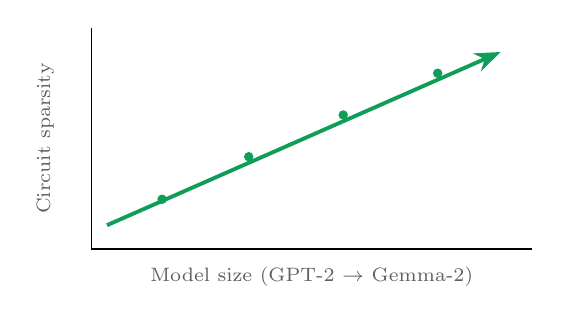
\begin{tikzpicture}
\draw[color=black, line width=0.5pt] (0,0) -- (5.6,0);
\draw[color=black, line width=0.5pt] (0,0) -- (0,2.8);
\node[below, font=\scriptsize, color=inkDim] at (2.8,-0.1) {Model size\ (GPT-2\ $\to$\ Gemma-2)};
\node[rotate=90, above, font=\scriptsize, color=inkDim] at (-0.35,1.4) {Circuit sparsity};
\draw[accentGreen, line width=1.4pt, -{Stealth}] (0.2,0.3) -- (5.2,2.5);
\fill[accentGreen] (0.9,0.63) circle (0.06);
\fill[accentGreen] (2.0,1.17) circle (0.06);
\fill[accentGreen] (3.2,1.70) circle (0.06);
\fill[accentGreen] (4.4,2.23) circle (0.06);
\end{tikzpicture}
\end{center}
\end{minipage}%
\hfill
\begin{minipage}[t]{0.58\linewidth}
\vspace{8pt}
\textbf{Claim.} Algorithmic circuits remain \textbf{localised in low-rank
singular directions as models scale}. Bigger models are not more diffuse ---
they are \emph{more} sparse in the SVD basis.

\vspace{4pt}
\textit{Why it matters for the Compass project.} If this holds, the same
scan-and-ablate recipe we demonstrated on GPT-2 / Phi-3 / Gemma-2 / Llama-3.2
should keep working on larger models, with equal or smaller $\alpha$ budgets.
\end{minipage}
\end{tcolorbox}

\end{document}
